% This LaTeX was auto-generated from MATLAB code.
% To make changes, update the MATLAB code and export to LaTeX again.

\documentclass{article}

\usepackage[utf8]{inputenc}
\usepackage[T1]{fontenc}
\usepackage{lmodern}
\usepackage{graphicx}
\usepackage{color}
\usepackage{hyperref}
\usepackage{amsmath}
\usepackage{amsfonts}
\usepackage{epstopdf}
\usepackage[table]{xcolor}
\usepackage{matlab}
\usepackage[paperheight=795pt,paperwidth=614pt,top=72pt,bottom=72pt,right=72pt,left=72pt,heightrounded]{geometry}

\sloppy
\epstopdfsetup{outdir=./}
\graphicspath{ {./hw9_media/} }

\begin{document}

\title{Homework 9: Truncated SVD, Tikhonov Regularization, and Solutions to Least Squares}
\author{Matthew Luyten\\
ECE6250}

\maketitle

\matlabheading{Problem 8.1}

\vspace{1em}
\begin{par}
\begin{flushleft}
This week, we learned new techniques to optimally solve least-squares problems. In the case of rank-deficient matrices,
the traditional pseudo-inverse least-squares solution does not minimize mean-squared error. Techniques like the truncated
SVD and Tikhonov Regularization allow us to perform low-rank approximations and develop a solution that minimizes
MSE for rank-deficient matrices. The truncated SVD is simple to implement, as you only have to truncate the N smallest
singular values from the matrix to form the approximation. However, this is only convenient if the SVD is already
available. Tikhonov Regularization solves this problem, since it does not require the SVD. It may be, however,
more inconvenient to determine a $\delta$ that produces the MMSE solution.
\end{flushleft}
\end{par}

\newpage

\matlabheading{Problem 9.2}

\begin{par}
\begin{flushleft}
$\hat{\mathbf{x}} ={\mathbf{A}}^{\dagger} \mathbf{b}={\left\lbrack \begin{array}{cccc}
0\ldotp 54 & 2\ldotp 4 & 3\ldotp 09 & 3\ldotp 73
\end{array}\right\rbrack }^T$, which is quite different from $\mathbf{x}={\left\lbrack \begin{array}{cccc}
1 & 2 & 3 & 4
\end{array}\right\rbrack }^T$. In fact, the MSE $||\mathit{\mathbf{x}}-\hat{\mathit{\mathbf{x}}} ||_2^2 =0\ldotp 27$, despite the fact that $\mathbf{Ax}=\mathbf{A}\hat{\mathbf{x}} =\mathbf{b}$. The matrix A is under-determined, so there are many solutions to $\mathbf{Ax}=\mathbf{b}$.
\end{flushleft}
\end{par}

\begin{matlabcode}
A = [[1, 4, 5, 6]; [6, 7, 2, 1]];
b = [48, 30].';
[u, s, v] = svd(A);
A_dag = v(:, 1:2)*inv(s(:, 1:2))*u.';
x_hat = A_dag*b;
display(x_hat);
\end{matlabcode}
\begin{matlaboutput}
x_hat = 4x1    
    0.5442
    2.4027
    3.0929
    3.7301

\end{matlaboutput}
\begin{matlabcode}
x = [1 2 3 4].';
A*x_hat;
fprintf("MSE of x: %d", norm((x-x_hat).^2));
\end{matlabcode}
\begin{matlaboutput}
MSE of x: 2.735177e-01
\end{matlaboutput}

\newpage

\matlabheading{Problem 9.4}

\begin{matlabcode}
load("blocksdeconv2024.mat");
\end{matlabcode}

\begin{par}
\begin{flushleft}
\textit{Part A} - Write a function that take vector $\mathbf{h}$ and returns an MxN circulant matrix $\mathbf{A}$ such that for any $\mathbf{x}\in {\mathbb{R}}^N$,  $\mathbf{Ax}$ is the vector of non-zero values of $\mathbf{h}$ convolved with $\mathbf{x}$
\end{flushleft}
\end{par}

\begin{matlabcode}
function A = generateCirculantMatrix(x, N)
    A = convmtx(x, N);
end
\end{matlabcode}


\begin{par}
\begin{flushleft}
\textit{Part B} - Find the SVD of $\mathbf{A}$. What are it's largest and smallest singular values? Calculate and plot ${\mathbf{A}}^{\dagger} \mathbf{y}$.
\end{flushleft}
\end{par}

\begin{par}
\begin{flushleft}
The largest singular value of $\mathbf{A}$is 0.9937.
\end{flushleft}
\end{par}

\begin{par}
\begin{flushleft}
The smallest singular value of $\mathbf{A}$ 0.0004.
\end{flushleft}
\end{par}

\begin{par}
\begin{flushleft}
See plot below:
\end{flushleft}
\end{par}

\begin{matlabcode}
A = generateCirculantMatrix(h, length(x));
[u, s, v] = svd(A);

A_dag = pinv(A);
x_hat = A_dag*y;
plot(x_hat);
title("Plot of $A^\dag y$ Noise-less Reconstruction", 'Interpreter','latex');
\end{matlabcode}
\begin{center}
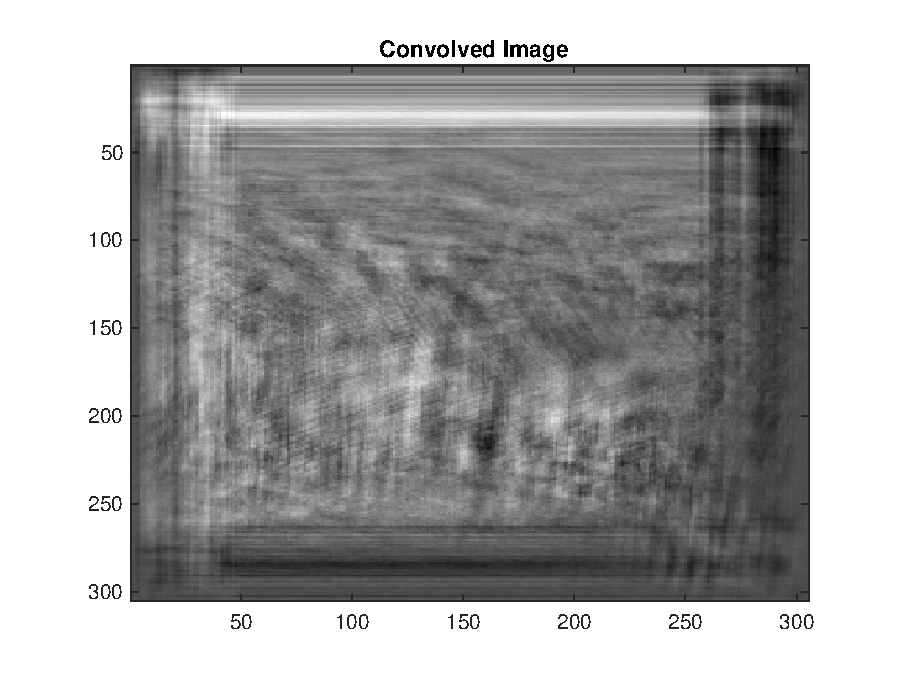
\includegraphics[width=\maxwidth{56.196688409433015em}]{figure_0.eps}
\end{center}
\begin{matlabcode}
fprintf("Largest SV: %d", max(s(:, 1)));
\end{matlabcode}
\begin{matlaboutput}
Largest SV: 9.993705e-01
\end{matlaboutput}
\begin{matlabcode}
fprintf("Smallest SV: %d", max(s(:, end)));
\end{matlabcode}
\begin{matlaboutput}
Smallest SV: 4.349731e-04
\end{matlaboutput}


\begin{par}
\begin{flushleft}
\textit{Part C} - Apply ${\mathbf{A}}^{\dagger}$ to the noisy ${\mathbf{y}}_{\mathbf{n}}$. Plot it and calculare the mean-square error and compare it to the measurement error.
\end{flushleft}
\end{par}

\begin{par}
$$||\mathit{\mathbf{x}}-\hat{\mathit{\mathbf{x}}} |_2^2 =5217\ldotp 225$$
\end{par}

\begin{par}
$$||\mathit{\mathbf{y}}-{\mathit{\mathbf{y}}}_{\mathit{\mathbf{n}}} ||_2^2 =0\ldotp 016$$
\end{par}

\begin{par}
\begin{flushleft}
The MSE is more than 300,000 times more than the measurement error!
\end{flushleft}
\end{par}

\begin{par}
\begin{flushleft}
See plot below:
\end{flushleft}
\end{par}

\begin{matlabcode}
xn_hat = A_dag*yn;
p1 = plot(xn_hat); hold on;
p2 = plot(x); hold off;
title("Original Signal vs Pseudo-Inverse Noisy Reconstruction", 'Interpreter','latex');
legend([p1, p2], ["$A^\dag y$", "x"], 'Interpreter','latex');
\end{matlabcode}
\begin{center}
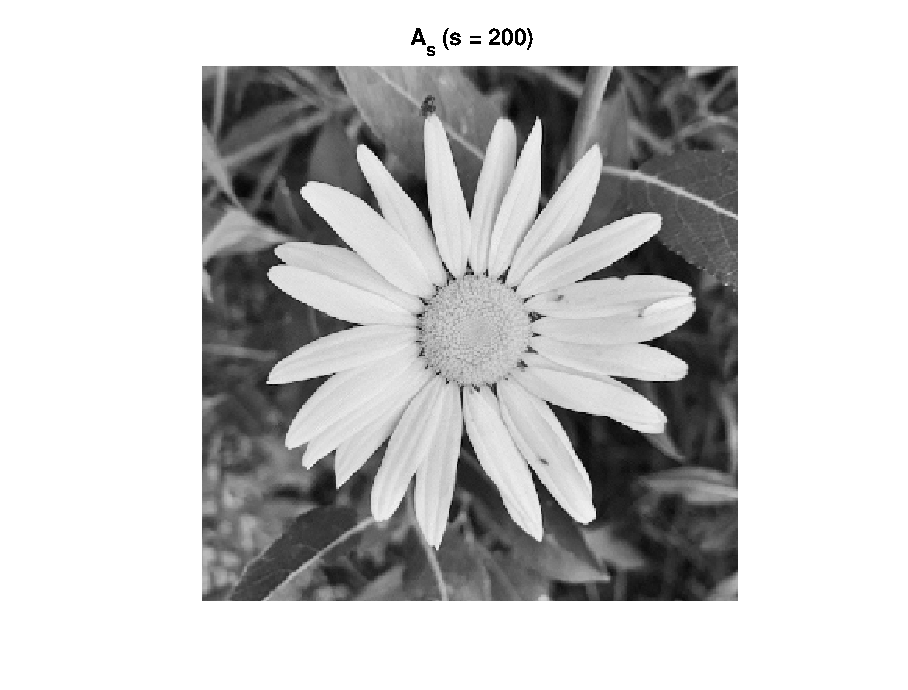
\includegraphics[width=\maxwidth{56.196688409433015em}]{figure_1.eps}
\end{center}
\begin{matlabcode}

fprintf("MSE of x: %d", norm((x-xn_hat).^2));
\end{matlabcode}
\begin{matlaboutput}
MSE of x: 5.217225e+03
\end{matlaboutput}
\begin{matlabcode}
fprintf("MSE of y: %d", norm((y-yn).^2));
\end{matlabcode}
\begin{matlaboutput}
MSE of y: 1.555198e-02
\end{matlaboutput}


\begin{par}
\begin{flushleft}
\textit{Part D} - Form an approximation  by truncating the last q terms of the singular values. Which q minimizes MSE?
\end{flushleft}
\end{par}

\begin{matlabcode}
function y = svd_trunc(x, r)
    [U, S, V] = svd(x);
    y = U(:,1:r)*S(1:r,1:r)*V(:,1:r).';
end
\end{matlabcode}


\begin{par}
\begin{flushleft}
Minimized $||\mathit{\mathbf{x}}-\hat{\mathit{\mathbf{x}}} |_2^2 =63\ldotp 5557$
\end{flushleft}
\end{par}

\begin{par}
\begin{flushleft}
q that minimizes $||\mathit{\mathbf{x}}-\hat{\mathit{\mathbf{x}}} |_2^2$: $q=379$
\end{flushleft}
\end{par}

\begin{par}
\begin{flushleft}
This minimization reduces the rank of $\mathbf{A}$ signficantly.
\end{flushleft}
\end{par}

\begin{par}
\begin{flushleft}
See plot of reconstructed signal.
\end{flushleft}
\end{par}

\begin{matlabcode}
error = zeros(512, 1);
for q = 1:512
    A_trunc = svd_trunc(A, 512-q);
    error(q) = norm((x-pinv(A_trunc)*yn).^2); 
end

[val, pos] = min(error);
A_trunc = svd_trunc(A, 512-pos);

p1 = plot(pinv(A_trunc)*yn); hold on;
p2 = plot(x); hold off;
title("Original Signal vs Pseudo-Inverse Noisy Reconstruction w/ Truncated SVD", 'Interpreter','latex');
legend([p1, p2], ["$A'^\dag y$", "x"], 'Interpreter','latex');
\end{matlabcode}
\begin{center}
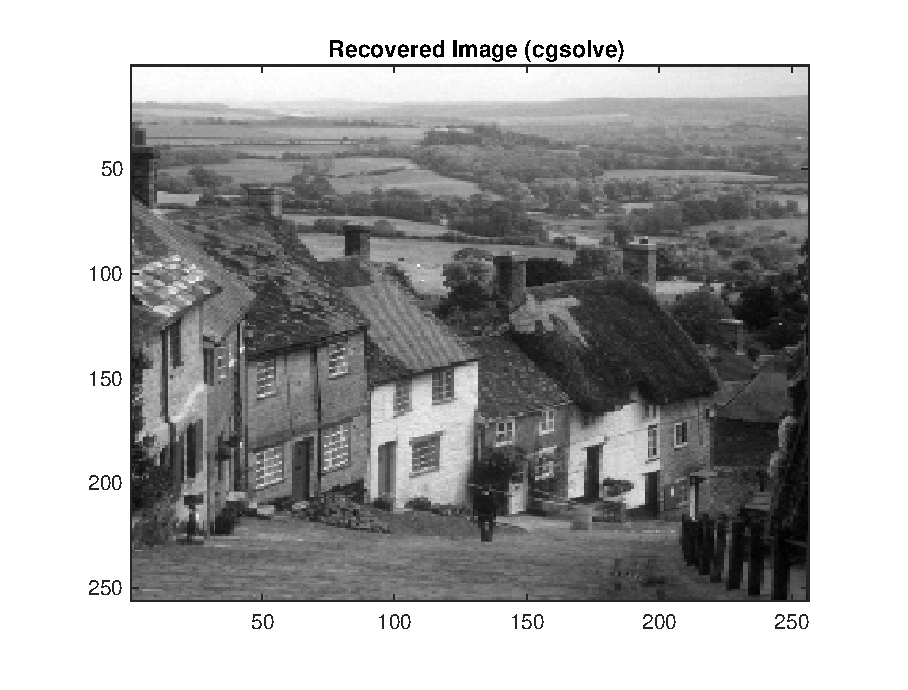
\includegraphics[width=\maxwidth{56.196688409433015em}]{figure_2.eps}
\end{center}
\begin{matlabcode}
fprintf("q that minimizes MSE: %i", pos);
\end{matlabcode}
\begin{matlaboutput}
q that minimizes MSE: 379
\end{matlaboutput}
\begin{matlabcode}
fprintf("MSE is %d", val);
\end{matlabcode}
\begin{matlaboutput}
MSE is 6.355575e+01
\end{matlaboutput}


\begin{par}
\begin{flushleft}
\textit{Part E }- Form another approximate inverse using Tikhonov Regularization. Try a number of values of $\delta$ which may minimize $||\mathit{\mathbf{x}}-\hat{\mathit{\mathbf{x}}} ||_2^2$. Calculate MSE.
\end{flushleft}
\end{par}

\begin{par}
$$||\mathit{\mathbf{x}}-\hat{\mathit{\mathbf{x}}} |_2^2 =63\ldotp 2332$$
\end{par}

\begin{par}
\begin{flushleft}
$\delta =\;$0.000081818
\end{flushleft}
\end{par}

\begin{par}
\begin{flushleft}
See plot below:
\end{flushleft}
\end{par}

\begin{matlabcode}
% This is the range of the minimum & was found experimentally
sigma = linspace(0, 0.0001, 100);
error = zeros(length(sigma), 1);
for i = 1:length(sigma)
    x_tik = (A.'*A+(sigma(i))*eye(512))\A.'*yn;
    error(i) = norm((x-x_tik).^2);
end

[val, pos] = min(error);
x_tik = (A.'*A+(sigma(pos))*eye(512))\A.'*yn;
p1 = plot(x_tik); hold on;
p2 = plot(x); hold off;
title("Original Signal vs Pseudo-Inverse Noisy Reconstruction w/ Tikhonov Reg.", 'Interpreter','latex');
legend([p1, p2], ["$A_{TIK}^\dag y$", "x"], 'Interpreter','latex');
\end{matlabcode}
\begin{center}
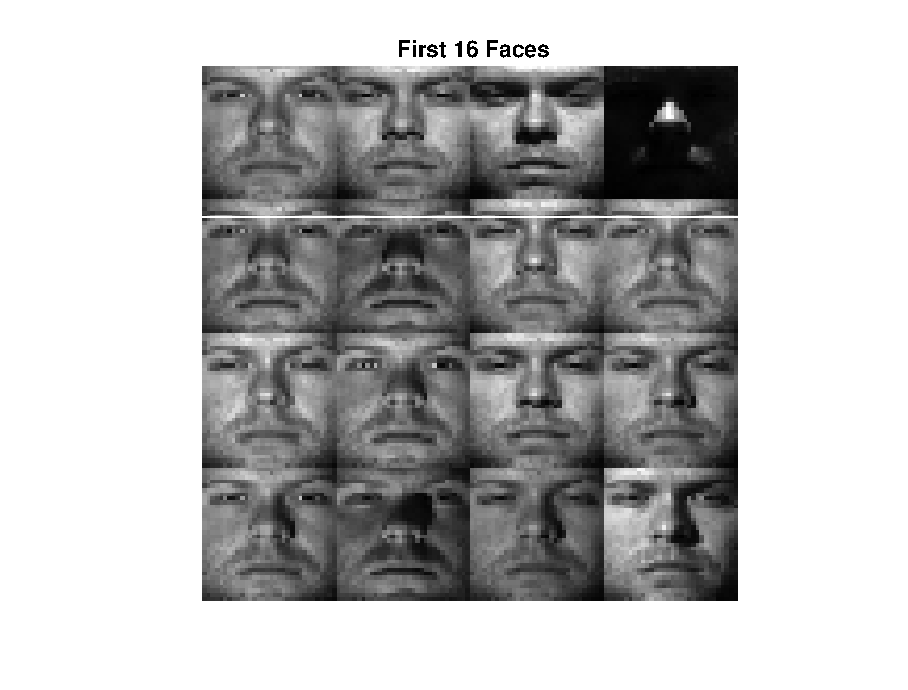
\includegraphics[width=\maxwidth{56.196688409433015em}]{figure_3.eps}
\end{center}
\begin{matlabcode}
fprintf("Sigma that minimizes MSE: %i", sigma(pos));
\end{matlabcode}
\begin{matlaboutput}
Sigma that minimizes MSE: 8.181818e-05
\end{matlaboutput}
\begin{matlabcode}
fprintf("MSE is %d", val);
\end{matlabcode}
\begin{matlaboutput}
MSE is 6.323320e+01
\end{matlaboutput}


\begin{par}
\begin{flushleft}
\textit{Part F }- Summarize your findinfs by comparing MSE in parts c, d, and e. Compare to the error of doing nothing.
\end{flushleft}
\end{par}

\begin{par}
\begin{flushleft}
The MSE of simply performing the pseudo-inverse is orders of magnitude worse than the minimized MSE using the truncated SVD or tikhonov regularization. The MSE of optimal truncated SVD and Tikhonov regularization is functionally the same, though Tikhonov regularization was able to acheive a slightly smaller MSE.
\end{flushleft}
\end{par}

\begin{par}
\begin{flushleft}
While the plot of the ${\mathbf{y}}_{\mathbf{n}}$ vs $\mathbf{x}$ looks cleaner than the above plots, it's mean square error is 2 times worse than that of the methods in d and e. Doing nothing is, however, better than simply reconstructing with the pseudo-inverse. It also requires 0 computations.
\end{flushleft}
\end{par}

\begin{par}
$$||{\mathbf{y}}_{\mathbf{n}} -\hat{\mathbf{x}} ||_2^2 =128\ldotp 5728$$
\end{par}

\begin{matlabcode}
% Find error of doing nothing
offset = length(h) / 2;
yn_sig = yn(offset:end-offset);
p1 = plot(yn_sig); hold on;
p2 = plot(x); hold off;
title("Original Signal vs Convolved Signal", 'Interpreter','latex');
legend([p1, p2], ["$y_n$", "x"], 'Interpreter','latex');
\end{matlabcode}
\begin{center}
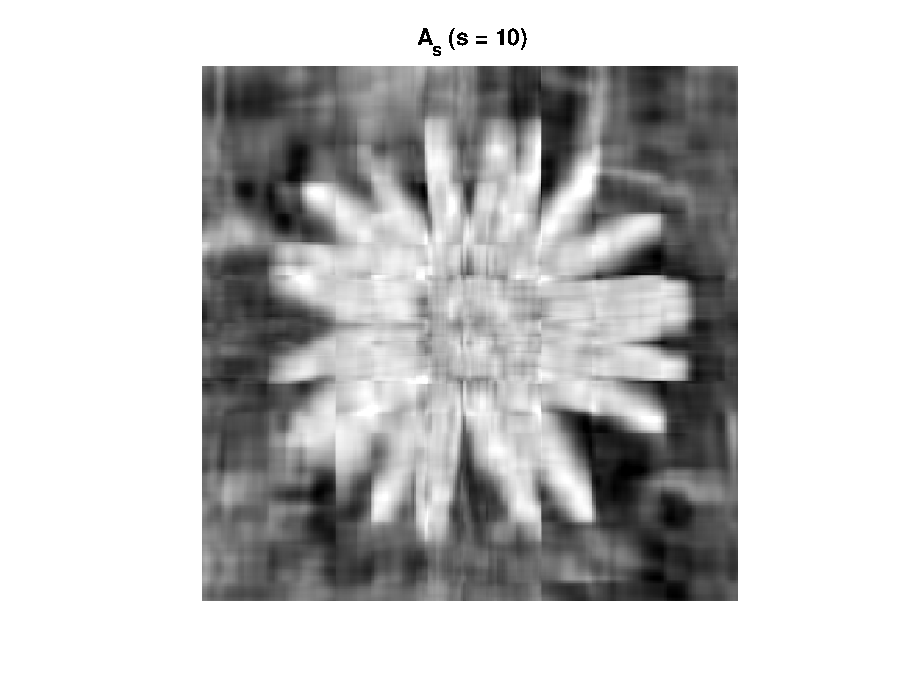
\includegraphics[width=\maxwidth{56.196688409433015em}]{figure_4.eps}
\end{center}
\begin{matlabcode}
fprintf("MSE of no reconstruction: %d", norm((x-yn_sig).^2));
\end{matlabcode}
\begin{matlaboutput}
MSE of no reconstruction: 1.285728e+02
\end{matlaboutput}

\end{document}
